\documentclass[12pt,a4paper]{report}

% ─── Packages ───────────────────────────────────────────────────────────────
\usepackage[utf8]{inputenc}
\usepackage[T1]{fontenc}
\usepackage[english]{babel}
\usepackage{geometry}
\usepackage{graphicx}
\usepackage{booktabs}
\usepackage{tabularx}
\usepackage{array}
\usepackage{longtable}
\usepackage{hyperref}
\usepackage{xcolor}
\usepackage{listings}
\usepackage{enumitem}
\usepackage{titlesec}
\usepackage{fancyhdr}
\usepackage{setspace}
\usepackage{parskip}
\usepackage{tcolorbox}
\usepackage{amsmath}
\usepackage{amssymb}
\usepackage{tikz}
\usetikzlibrary{shapes.geometric, arrows, positioning, fit, calc}
\usepackage{mdframed}
\usepackage{float}

% ─── Page Layout ────────────────────────────────────────────────────────────
\geometry{
  top=2.5cm, bottom=2.5cm,
  left=3cm,  right=2.5cm,
  headheight=15pt
}

% ─── Colors ─────────────────────────────────────────────────────────────────
\definecolor{primary}{HTML}{0A3D62}
\definecolor{accent}{HTML}{FF6B35}
\definecolor{lightgray}{HTML}{F4F4F4}
\definecolor{codebg}{HTML}{F8F8F8}
\definecolor{codeframe}{HTML}{CCCCCC}

% ─── Hyperref Setup ─────────────────────────────────────────────────────────
\hypersetup{
  colorlinks=true,
  linkcolor=primary,
  urlcolor=accent,
  citecolor=primary
}

% ─── Section Formatting ─────────────────────────────────────────────────────
\titleformat{\chapter}[display]
  {\normalfont\huge\bfseries\color{primary}}
  {\chaptertitlename\ \thechapter}{20pt}{\Huge}
\titleformat{\section}
  {\normalfont\Large\bfseries\color{primary}}
  {\thesection}{1em}{}
\titleformat{\subsection}
  {\normalfont\large\bfseries\color{primary!80!black}}
  {\thesubsection}{1em}{}

% ─── Header / Footer ────────────────────────────────────────────────────────
\pagestyle{fancy}
\fancyhf{}
\fancyhead[L]{\small\textit{JeunesseActive -- Software Architecture Report}}
\fancyhead[R]{\small\textit{Spring 2026}}
\fancyfoot[C]{\thepage}
\renewcommand{\headrulewidth}{0.4pt}

% ─── Code Listings ──────────────────────────────────────────────────────────
\lstset{
  backgroundcolor=\color{codebg},
  frame=single,
  rulecolor=\color{codeframe},
  basicstyle=\ttfamily\small,
  breaklines=true,
  numbers=left,
  numberstyle=\tiny\color{gray},
  keywordstyle=\color{primary}\bfseries,
  commentstyle=\color{gray}\itshape,
  stringstyle=\color{accent},
  tabsize=2,
}

% ─── Spacing ────────────────────────────────────────────────────────────────
\onehalfspacing

% ════════════════════════════════════════════════════════════════════════════
\begin{document}

% ─── Title Page ─────────────────────────────────────────────────────────────
\begin{titlepage}
\centering

\vspace*{1.5cm}
{\color{primary}\rule{\linewidth}{3pt}}
\vspace{0.5cm}

{\Huge\bfseries\color{primary} PROJECT REPORT}\\[0.5cm]
{\LARGE\bfseries Spring 2026 Software Architecture}

\vspace{0.5cm}
{\color{primary}\rule{\linewidth}{3pt}}
\vspace{1.5cm}

{\Huge\bfseries\color{accent} JeunesseActive}\\[0.4cm]
{\Large\textit{La Plateforme des Jeunes Entrepreneurs Africains}}\\[0.3cm]
{\large A GPS-Enabled Service Marketplace for African Youth Entrepreneurs}

\vspace{2cm}

\begin{tabular}{ll}
  \textbf{Course Code / Title:} & Software Architecture -- Spring 2026 \\[6pt]
  \textbf{Group Number:}        & Group 40 \\[6pt]
  \textbf{Project Topic:}       & Mobile Service Marketplace (Flutter + Node.js) \\[6pt]
  \textbf{GitHub Repository:}   & \url{https://github.com/Joy-chebs/Active-Youths.git} \\[6pt]
  \textbf{Group Leader:}        & [Joy Atehbih Chebegwen] \\
\end{tabular}

\vspace{1.5cm}

\begin{tcolorbox}[colback=primary!8, colframe=primary, title={\textbf{Group Information}}, coltitle=white]
\begin{tabularx}{\linewidth}{c X c c}
  \toprule
  \textbf{SN} & \textbf{Member's Name} & \textbf{Registration Number} & \textbf{Team Role} \\
  \midrule
  1 & [Joy Atehbih Chebegwen] & [ICTU20234316] & Scrum Master / Flutter Dev /  Backend Developer \\
  2 & [Leudjou Nguepleu Maxime] & [ICTU20234264] & Database / DevOps / UI/UX / Frontend Dev \\
  
  \bottomrule
\end{tabularx}
\end{tcolorbox}

\vfill
{\large\today}
\end{titlepage}

% ─── Table of Contents ──────────────────────────────────────────────────────
\tableofcontents
\newpage

% ════════════════════════════════════════════════════════════════════════════
%  CHAPTER ONE: INTRODUCTION
% ════════════════════════════════════════════════════════════════════════════
\chapter{Introduction}

% ── 1.1 General Introduction ─────────────────────────────────────────────
\section{General Introduction}

Africa's youth population represents one of the fastest-growing economic forces on the continent. Despite abundant skills and entrepreneurial spirit, young service providers—ranging from electricians and plumbers to tutors and graphic designers—often struggle to connect with clients efficiently. Existing platforms are either tailored to Western markets, require costly data connectivity, or lack the GPS-based discovery features that make local commerce practical.

\textbf{JeunesseActive} (Active Youths) is a cross-platform mobile application designed to bridge this gap. Built with Flutter for the frontend and Node.js (Express) for the backend, the platform provides a structured marketplace where youth entrepreneurs can publish service offers, build professional profiles, and be discovered by employers through an interactive GPS map. Employers can browse services by category, message providers directly, and leave reviews to build community trust.

The application is designed with the realities of African mobile usage in mind: offline-friendly local storage via \texttt{SharedPreferences}, efficient map rendering through OpenStreetMap (no Google Maps billing), and a clean bilingual-ready codebase.

% ── 1.2 Aim and Objectives ───────────────────────────────────────────────
\section{Aim and Objectives}

\subsection*{Aim}
To design and develop a mobile service marketplace that empowers African youth entrepreneurs to monetise their skills and connect with local employers through GPS-based discovery, professional profiles, and real-time messaging.

\subsection*{Objectives}
\begin{enumerate}[label=\textbf{O\arabic*.}]
  \item Implement a dual-role authentication system supporting both \textit{Prestataire} (service provider) and \textit{Employeur} (employer) account types, with JWT-based session management.
  \item Provide service providers with a complete profile management system including photo upload, skill listing, statistics (views, ratings), and service offer publication.
  \item Deliver employers an intuitive discovery interface (category search + GPS map) to locate nearby service providers.
  \item Implement a real-time direct messaging system between employers and service providers using Kafka-based event-driven architecture.
  \item Build a scalable RESTful backend using Express 5, Prisma ORM, and PostgreSQL, capable of supporting event-driven microservice expansion.
  \item Apply Scrum methodology throughout the project, ensuring iterative delivery, transparent sprint planning, and continuous quality improvement.
\end{enumerate}

% ── 1.3 Problem Statement ────────────────────────────────────────────────
\section{Problem Statement}

Young African service providers face three critical problems:

\begin{itemize}
  \item \textbf{Invisibility:} Skilled individuals rely on word-of-mouth or informal networks, making it nearly impossible for potential clients in adjacent areas to discover them.
  \item \textbf{Lack of credibility infrastructure:} Without a structured review system or verifiable professional profile, trust is difficult to establish, especially between strangers.
  \item \textbf{Communication friction:} No dedicated channel exists for immediate, in-context negotiation between a client who has spotted a service offer and the provider who published it.
\end{itemize}

JeunesseActive solves all three problems by combining a GPS-powered discovery map, a structured review and rating system, and an integrated direct messaging system within a single mobile application.

% ════════════════════════════════════════════════════════════════════════════
%  CHAPTER TWO: LITERATURE REVIEW
% ════════════════════════════════════════════════════════════════════════════
\chapter{Literature Review}

% ── 2.1 Software Development Methodologies ───────────────────────────────
\section{Software Development Methodologies}

Modern software projects typically adopt one of several development methodologies, each carrying distinct trade-offs in terms of planning rigour, adaptability, and team collaboration.

\subsection{Waterfall}
Waterfall is a sequential, plan-driven model where each phase (requirements, design, implementation, testing, deployment) must be completed before the next begins \cite{royce1970}. It works best when requirements are fully known upfront and changes are unlikely. Its primary weakness is inflexibility: late-discovered defects are expensive to fix.

\subsection{Agile}
Agile is an umbrella of iterative methodologies governed by the Agile Manifesto (2001), which prioritises individuals and interactions over processes and tools, working software over comprehensive documentation, customer collaboration over contract negotiation, and responding to change over following a plan \cite{beck2001}. Agile promotes short feedback loops and welcomes changing requirements even late in development.

\subsection{Scrum}
Scrum is the most widely adopted Agile framework \cite{schwaber2020}. It organises work into fixed-length \textit{Sprints} (typically 1–4 weeks), governed by three roles (Product Owner, Scrum Master, Development Team) and five events (Sprint Planning, Daily Scrum, Sprint Review, Sprint Retrospective, and the Sprint itself). Scrum artifacts—Product Backlog, Sprint Backlog, and Increment—provide transparency and enable empirical process control.

\subsection{Kanban}
Kanban visualises work as cards on a board with columns representing workflow states (e.g., To Do → In Progress → Done). It is flow-based rather than iteration-based, making it better suited for continuous delivery and support work than for greenfield development with evolving requirements.

\subsection{Extreme Programming (XP)}
XP emphasises technical excellence through practices such as test-driven development (TDD), pair programming, continuous integration, and refactoring. It is highly effective when code quality is critical but demands significant discipline from the team.

% ── 2.2 Comparison ───────────────────────────────────────────────────────
\section{Comparison between Different Software Development Methodologies}

\begin{table}[H]
\centering
\caption{Comparison of Software Development Methodologies}
\renewcommand{\arraystretch}{1.3}
\begin{tabularx}{\linewidth}{lXXXX}
\toprule
\textbf{Criterion} & \textbf{Waterfall} & \textbf{Scrum} & \textbf{Kanban} & \textbf{XP} \\
\midrule
Flexibility         & Low    & High   & Very High & High \\
Documentation       & Heavy  & Light  & Minimal   & Light \\
Team Structure      & Siloed & Roles  & Self-org  & Pairs \\
Feedback Cycle      & Long   & Short  & Continuous & Short \\
Best For            & Stable reqs & Evolving reqs & Ops/support & Quality-critical \\
Risk Management     & Late   & Per sprint & Ongoing & Continuous \\
\bottomrule
\end{tabularx}
\end{table}

% ── 2.3 Reason for Scrum ─────────────────────────────────────────────────
\section{Reason for the Choice of Scrum Methodology}

Scrum was selected for JeunesseActive for several compounding reasons:

\begin{enumerate}
  \item \textbf{Evolving requirements:} A marketplace application targeting a novel user segment (African youth entrepreneurs) has inherently uncertain requirements. Scrum's iterative nature allows the team to validate assumptions each sprint rather than committing to a fixed specification.
  \item \textbf{Time-boxed delivery:} The academic deadline creates a natural constraint that aligns well with Scrum's Sprint cadence. Each Sprint delivers a potentially shippable increment.
  \item \textbf{Role clarity:} With four team members playing distinct roles (Scrum Master, Product Owner, Backend, Frontend), Scrum's role definitions prevent scope conflicts and establish accountability.
  \item \textbf{Transparency:} Scrum artifacts (Product Backlog, Sprint Backlog) make the state of the project visible to all stakeholders, including the project supervisor.
  \item \textbf{Continuous quality:} Sprint reviews and retrospectives embed quality feedback loops throughout the development cycle.
\end{enumerate}

% ── 2.4 General Review ───────────────────────────────────────────────────
\section{General Review of Related Concepts}

\subsection{Event-Driven Architecture (EDA)}
EDA is a design paradigm in which system components communicate by producing and consuming events. Components are decoupled: a producer publishes an event to a message broker (Apache Kafka in our case) without knowing which consumers will react to it. This enables horizontal scalability and resilience \cite{fowler2017}.

\subsection{GPS and Location-Based Services (LBS)}
LBS applications leverage device GPS hardware to provide location-aware features. OpenStreetMap (OSM) is the open-source equivalent of Google Maps and powers the \texttt{flutter\_map} package used in JeunesseActive. OSM tiles are free to use, removing billing constraints for an early-stage startup application.

\subsection{RESTful API Design}
REST (Representational State Transfer) is an architectural style for distributed hypermedia systems. RESTful APIs use standard HTTP methods (GET, POST, PUT, DELETE) and status codes, making them intuitive for client developers and compatible with all HTTP-capable clients.

% ── 2.5 Related Literature ───────────────────────────────────────────────
\section{Review of Related Literature}

\subsection{Comparable Platforms}
\begin{itemize}
  \item \textbf{Upwork / Fiverr:} Global freelancing platforms that pioneered the digital service marketplace concept. They lack GPS proximity search and are not tailored for informal-economy service providers in Africa.
  \item \textbf{Taskrabbit:} Offers location-based task assignment but operates only in Western markets and does not support the employee-employer dual-role model we implement.
  \item \textbf{Jumia:} An African e-commerce leader, but focused on product sales rather than services, and lacks real-time messaging between providers and buyers.
  \item \textbf{Lynk (Kenya):} The closest comparable—a Kenyan platform connecting skilled workers with employers. JeunesseActive differentiates through open-source stack choices, GPS-first discovery, and a Flutter cross-platform approach.
\end{itemize}

\subsection{Technical Literature}
\begin{itemize}
  \item \textbf{Kafka for real-time data:} Confluent's white papers on Kafka streaming confirm its suitability for low-latency event pipelines, which we use for notifications and messaging events \cite{kafka2021}.
  \item \textbf{Flutter performance:} Google's Flutter documentation establishes the framework's suitability for high-performance mobile UI with a single codebase targeting both Android and iOS \cite{flutter2023}.
  \item \textbf{Prisma ORM:} Prisma's type-safe query builder reduces SQL injection risk and accelerates schema-driven development in TypeScript backends \cite{prisma2024}.
\end{itemize}

% ════════════════════════════════════════════════════════════════════════════
%  CHAPTER THREE: METHODOLOGY AND MATERIALS
% ════════════════════════════════════════════════════════════════════════════
\chapter{Methodology and Materials}

% ── 3.1 Research Methodology ─────────────────────────────────────────────
\section{Research Methodology}

The project followed a \textbf{Design Science Research} approach: the team iteratively designed, built, and evaluated an artefact (the JeunesseActive application) against real-world requirements. Each Sprint served as a micro-research cycle: hypotheses about user needs were encoded as user stories, implemented as features, and validated through internal review and test execution.

% ── 3.2 System Requirements ──────────────────────────────────────────────
\section{System Requirements}

\subsection{Functional Requirements}

\begin{longtable}{lp{10cm}}
\toprule
\textbf{ID} & \textbf{Requirement} \\
\midrule
FR-01 & A user shall be able to register as either a \textit{Prestataire} or \textit{Employeur}. \\
FR-02 & A user shall be able to log in with email/password or social providers (Google, Facebook). \\
FR-03 & A Prestataire shall be able to create, edit, and delete service offers with title, category, price type, location, and images. \\
FR-04 & An Employeur shall be able to browse and filter service offers by category. \\
FR-05 & Both user types shall be able to view an interactive GPS map displaying nearby service providers and employers. \\
FR-06 & Users shall be able to initiate and participate in direct messaging conversations. \\
FR-07 & Users shall be able to leave reviews and star ratings on other users' profiles. \\
FR-08 & Users shall receive push notifications for new messages and nearby searches. \\
FR-09 & A Prestataire shall be able to view profile statistics (views, rating, review count). \\
FR-10 & Users shall be able to upload a profile photo from the camera or gallery. \\
\bottomrule
\end{longtable}

\subsection{Non-Functional Requirements}

\begin{longtable}{lp{10cm}}
\toprule
\textbf{ID} & \textbf{Requirement} \\
\midrule
NFR-01 & \textbf{Performance:} API responses shall complete within 500ms under normal load. \\
NFR-02 & \textbf{Security:} Passwords shall be hashed with bcrypt (cost factor 10); all routes except auth shall require a valid JWT. \\
NFR-03 & \textbf{Scalability:} The backend shall be event-driven (Kafka) to allow future microservice decomposition without breaking existing clients. \\
NFR-04 & \textbf{Reliability:} The database schema shall enforce referential integrity with cascading deletes. \\
NFR-05 & \textbf{Usability:} The UI shall follow a consistent design system (Navy \texttt{\#0A3D62} + Orange \texttt{\#FF6B35}, Poppins font). \\
NFR-06 & \textbf{Portability:} The mobile app shall run on Android (API 21+) and iOS (12+) from a single codebase. \\
NFR-07 & \textbf{Maintainability:} All backend code shall be TypeScript with strict mode enabled. \\
\bottomrule
\end{longtable}

% ── 3.3 System Design ────────────────────────────────────────────────────
\section{System Design}

\subsection{Architecture of the System (High-Level Design)}

JeunesseActive follows a \textbf{client-server architecture} with an event-driven backend extension layer.

\begin{figure}[H]
\centering
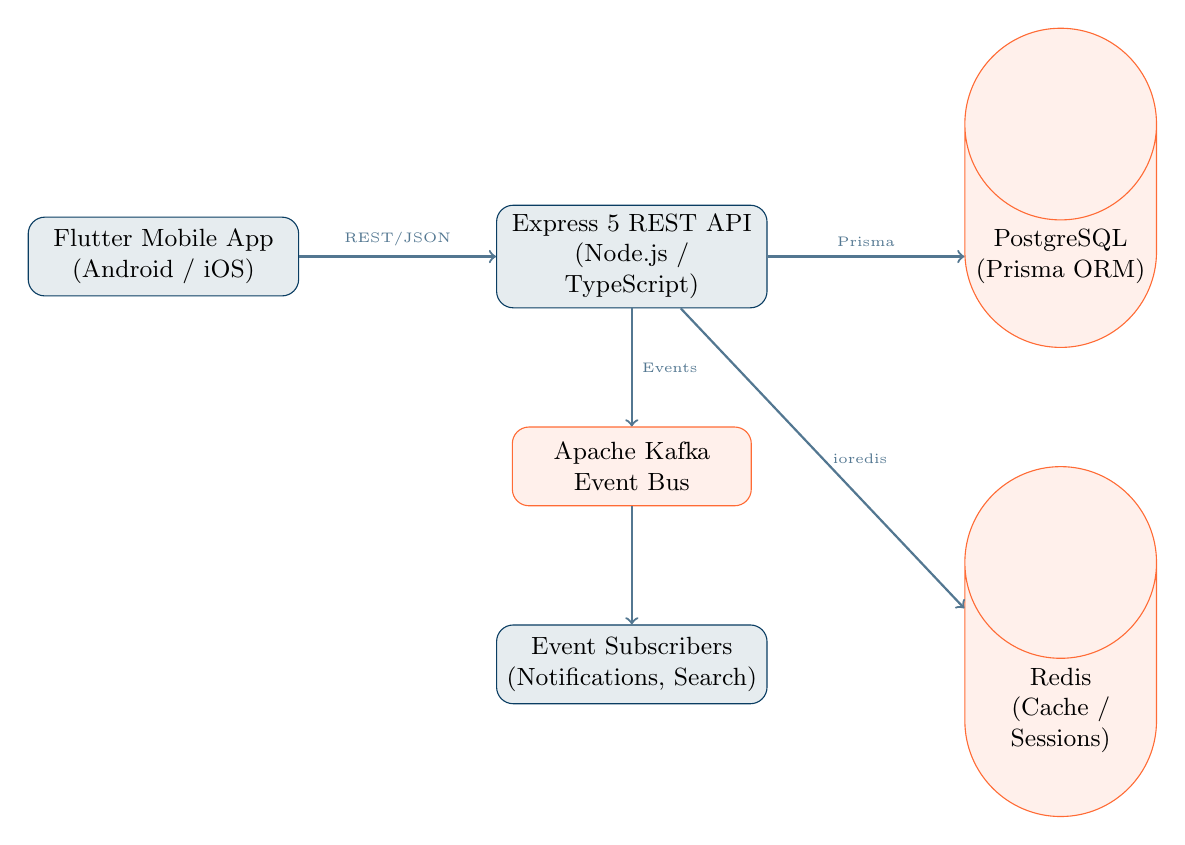
\begin{tikzpicture}[
  node distance=1.2cm and 2cm,
  box/.style={rectangle, rounded corners=6pt, draw=primary, fill=primary!10, text width=3.2cm, align=center, minimum height=1cm, font=\small},
  db/.style={cylinder, shape border rotate=90, draw=accent, fill=accent!10, text width=2.2cm, align=center, minimum height=1.2cm, font=\small},
  arrow/.style={->, thick, color=primary!70},
  event/.style={rectangle, rounded corners=6pt, draw=accent, fill=accent!10, text width=2.8cm, align=center, minimum height=1cm, font=\small}
]

% Flutter App
\node[box] (flutter) {Flutter Mobile App\\(Android / iOS)};

% Express API
\node[box, right=2.5cm of flutter] (api) {Express 5 REST API\\(Node.js / TypeScript)};

% Kafka
\node[event, below=1.5cm of api] (kafka) {Apache Kafka\\Event Bus};

% PostgreSQL
\node[db, right=2.5cm of api] (pg) {PostgreSQL\\(Prisma ORM)};

% Redis
\node[db, below=1.5cm of pg] (redis) {Redis\\(Cache / Sessions)};

% Subscribers
\node[box, below=1.5cm of kafka] (subs) {Event Subscribers\\(Notifications, Search)};

% Arrows
\draw[arrow] (flutter) -- node[above, font=\tiny]{REST/JSON} (api);
\draw[arrow] (api) -- node[above, font=\tiny]{Prisma} (pg);
\draw[arrow] (api) -- node[right, font=\tiny]{Events} (kafka);
\draw[arrow] (kafka) -- (subs);
\draw[arrow] (api) -- node[right, font=\tiny]{ioredis} (redis);

\end{tikzpicture}
\caption{High-Level System Architecture of JeunesseActive}
\end{figure}

\subsubsection{Layer Descriptions}
\begin{itemize}
  \item \textbf{Presentation Layer (Flutter):} The mobile application renders screens, manages local state via Provider, and persists authentication tokens and demo data using SharedPreferences.
  \item \textbf{API Layer (Express 5):} A modular Node.js server organised by feature modules (\texttt{auth}, \texttt{services}, \texttt{messages}, etc.). Each module contains its own controller, service, and route files. JWT middleware protects all non-public endpoints.
  \item \textbf{Data Layer (PostgreSQL + Prisma):} The relational database stores all persistent data. Prisma provides type-safe query building and handles schema migrations.
  \item \textbf{Event Layer (Kafka):} After state-changing operations (user registration, listing creation, message sent), the API publishes events to Kafka topics. Dedicated consumer groups process these events asynchronously (e.g., triggering notifications).
  \item \textbf{Cache Layer (Redis via ioredis):} Used for session caching and frequently-read data to reduce database load.
\end{itemize}


% System boundary
\draw[primary!60, thick] (0,0) rectangle (9,8);
\node[font=\small\bfseries, color=primary] at (4.5,8.3) {JeunesseActive System};

% Actors
\node[actor] (prest) at (-1.5,6.5) {Prestataire};
\node[actor] (emp)   at (-1.5,1.5) {Employeur};
\node[actor] (sys2)  at (10.5,4)   {System};

% UML Diagram
\subsubsection{Use Case Diagram}

\textbf{Actors:}
\begin{itemize}[noitemsep]
  \item \textbf{Service Provider} -- Registered user with \texttt{userType = employee}
  \item \textbf{Employer} -- Registered user with \texttt{userType = employer}
  \item \textbf{System (Kafka Consumer)} -- Internal automated actor
\end{itemize}

\begin{tcolorbox}[noteboxstyle, title={Use Cases -- Service Provider}]
\begin{itemize}[noitemsep, leftmargin=*]
  \item UC-SP-01: Register / Login (email+password or OAuth)
  \item UC-SP-02: Create / Edit / Delete service offer
  \item UC-SP-03: Upload service images (up to 5 via Cloudinary)
  \item UC-SP-04: Upload/change profile photo
  \item UC-SP-05: View dashboard statistics (offers, views, rating, reviews)
  \item UC-SP-06: Send and receive direct messages
  \item UC-SP-07: Receive push notifications
  \item UC-SP-08: View and manage profile (bio, skills, GPS location)
\end{itemize}
\end{tcolorbox}

\begin{tcolorbox}[warningboxstyle, title={Use Cases -- Employer}]
\begin{itemize}[noitemsep, leftmargin=*]
  \item UC-EM-01: Register / Login (email+password or OAuth)
  \item UC-EM-02: Browse/search service listings (keyword, category, GPS radius)
  \item UC-EM-03: View service detail and provider profile
  \item UC-EM-04: Contact a provider (initiate conversation)
  \item UC-EM-05: View GPS map with provider markers (OpenStreetMap)
  \item UC-EM-06: Receive AI-style service recommendations
  \item UC-EM-07: Submit rating and review for a provider
  \item UC-EM-08: Receive push notifications for messages
\end{itemize}
\end{tcolorbox}

\subsubsection{Class Diagram (Domain Model)}

The core domain classes and their principal associations in the system are:

\begin{verbatim}
 ┌─────────────────────────────┐
 │           User              │
 ├─────────────────────────────┤
 │ id: UUID (PK)               │
 │ name, email, phone          │
 │ password?: string           │
 │ userType: employee|employer │
 │ latitude?, longitude?       │
 │ skills: string[]            │
 │ rating: float               │
 │ isVerified: boolean         │
 │ companyName?: string        │
 └─────────┬──────────────┬───┘
           │ 1:N          │ 1:N
   ┌───────▼──────┐  ┌────▼─────────────┐
   │ ServiceOffer │  │     Review        │
   ├──────────────┤  ├───────────────────┤
   │ id: UUID     │  │ id, reviewerId    │
   │ userId (FK)  │  │ targetUserId (FK) │
   │ title, desc  │  │ rating (1-5)      │
   │ category     │  │ comment           │
   │ price, type  │  └───────────────────┘
   │ images[]     │
   │ viewCount    │      User M:N User (through Conversation)
   └──────────────┘
                          ┌──────────────────┐
                          │  Conversation    │
                          ├──────────────────┤
                          │ user1Id, user2Id │
                          │ lastMessage      │
                          │ unreadCount      │
                          └────────┬─────────┘
                                   │ 1:N
                          ┌────────▼─────────┐
                          │    Message       │
                          ├──────────────────┤
                          │ conversationId   │
                          │ senderId         │
                          │ receiverId       │
                          │ content, isRead  │
                          └──────────────────┘
\end{verbatim}

\subsubsection{Sequence Diagram -- Service Creation with Kafka Event}

\begin{verbatim}
Flutter App       API (listings)    Prisma (DB)        Kafka Broker
    │                  │                 │                   │
    │ POST /api/services (JWT + body) ──>│                   │
    │                  │── INSERT INTO ServiceOffer ─────>  │
    │                  │<── ServiceOffer object ───────────  │
    │                  │── publishListingCreated() ───────────────────>│
    │<── 201 + service─│                 │                   │
    │                  │                 │            listingSubscriber
    │                  │                 │<── consume(listing.created)─│
    │                  │                 │     (update notification)   │
    │                  │                 │<── consume(listing.created)─│
    │                  │                 │     (update search index)   │
\end{verbatim}

\subsubsection{Sequence Diagram -- Recommendation Flow}

\begin{verbatim}
Flutter App       API (matching)    Search History   Prisma (DB)
    │                  │                 │                │
    │ GET search history ─────────────────────────────>  │
    │<── [term1, term2, ...] ─────────────────────────   │
    │                  │                 │                │
    │ POST /api/matching/recommendations │                │
    │   body: { searchHistory, limit } ─>│                │
    │                  │── findMany(ServiceOffer, isAvailable) ──────>│
    │                  │<── all available offers ──────────────────   │
    │                  │── score each offer (weighted algo) ──        │
    │                  │── sort descending, slice top N ──            │
    │<── 200 + ranked offers array ─────│                             │
\end{verbatim}


% Actor connections
\draw (prest) -- (reg); \draw (prest) -- (profile); \draw (prest) -- (pub); \draw (prest) -- (msg);
\draw (emp)   -- (reg); \draw (emp)   -- (browse);  \draw (emp)   -- (map);  \draw (emp)   -- (msg); \draw (emp) -- (review);
\draw (sys2)  -- (notify);

\end{tikzpicture}
\caption{Use Case Diagram -- JeunesseActive}
\end{figure}

\subsubsection{Entity-Relationship (ER) Diagram}

The database schema (defined via Prisma) consists of the following core entities and relationships:

\begin{figure}[H]
\centering
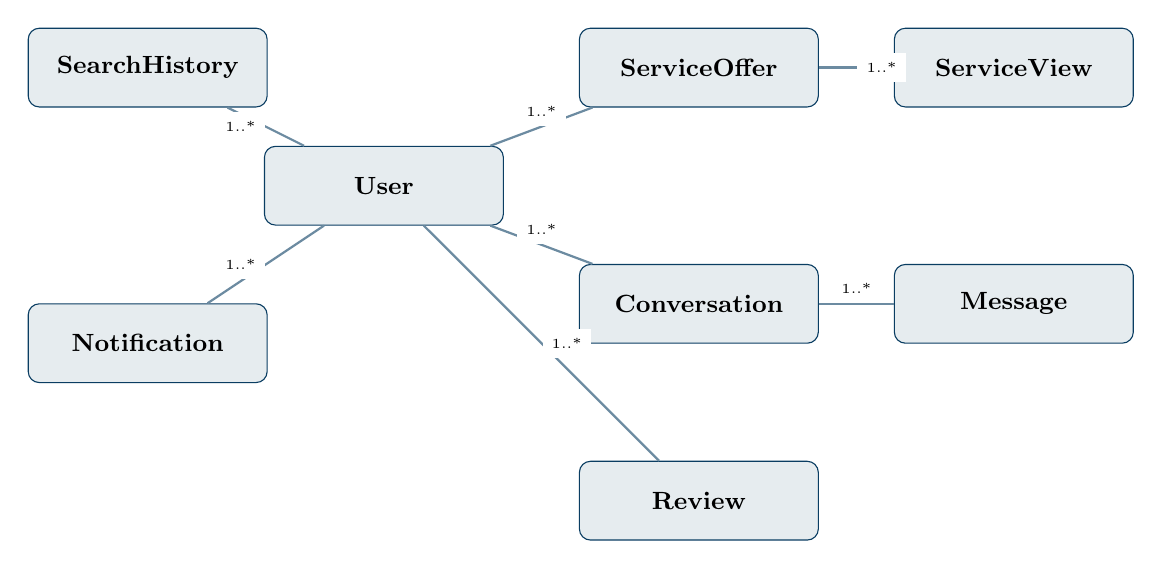
\begin{tikzpicture}[
  entity/.style={rectangle, draw=primary, fill=primary!10, rounded corners=4pt, text width=2.8cm, align=center, minimum height=1cm, font=\small\bfseries},
  rel/.style={draw=primary!60, thick},
  label/.style={font=\tiny, fill=white}
]
\node[entity] (user)    at (0,0)    {User};
\node[entity] (service) at (4,1.5)  {ServiceOffer};
\node[entity] (conv)    at (4,-1.5) {Conversation};
\node[entity] (msg)     at (8,-1.5) {Message};
\node[entity] (review)  at (4,-4)   {Review};
\node[entity] (notif)   at (-3,-2)  {Notification};
\node[entity] (search)  at (-3,1.5) {SearchHistory};
\node[entity] (view)    at (8,1.5)  {ServiceView};

\draw[rel] (user) -- node[label,above]{1..*} (service);
\draw[rel] (user) -- node[label,above]{1..*} (conv);
\draw[rel] (conv) -- node[label,above]{1..*} (msg);
\draw[rel] (user) -- node[label,right]{1..*} (review);
\draw[rel] (user) -- node[label,left]{1..*} (notif);
\draw[rel] (user) -- node[label,left]{1..*} (search);
\draw[rel] (service) -- node[label,right]{1..*} (view);
\end{tikzpicture}
\caption{Simplified ER Diagram -- JeunesseActive Database}
\end{figure}

\subsubsection{Sequence Diagram: User Registration Flow}

\begin{figure}[H]
\centering
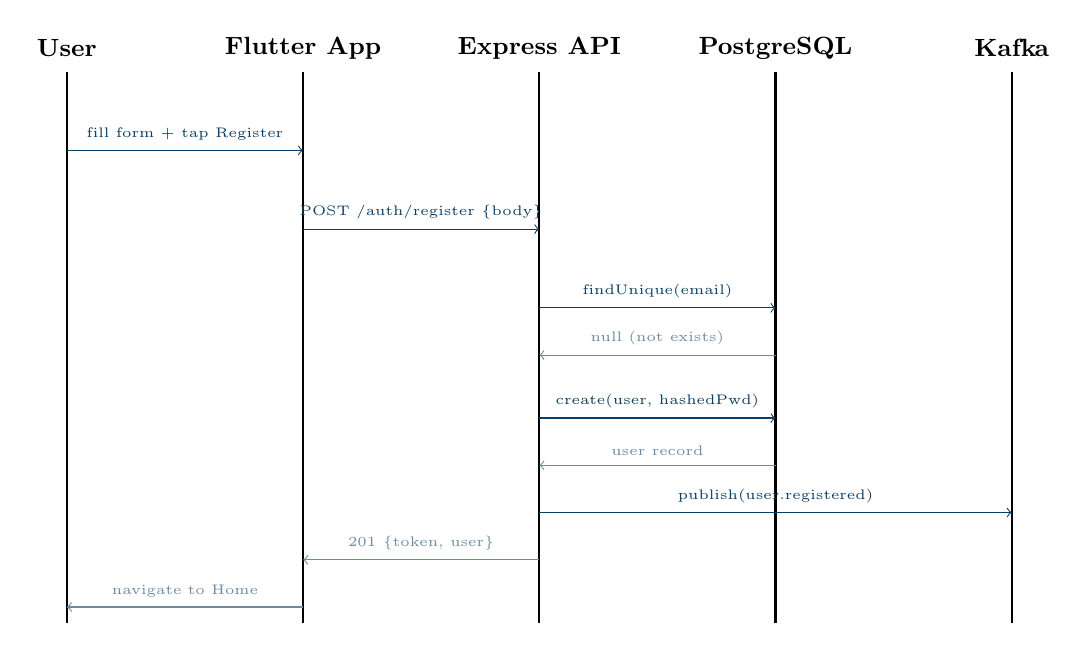
\begin{tikzpicture}[font=\small]
  % Lifelines
  \draw[thick] (0,0) -- (0,-7); \node at (0,0.3) {\textbf{User}};
  \draw[thick] (3,0) -- (3,-7); \node at (3,0.3) {\textbf{Flutter App}};
  \draw[thick] (6,0) -- (6,-7); \node at (6,0.3) {\textbf{Express API}};
  \draw[thick] (9,0) -- (9,-7); \node at (9,0.3) {\textbf{PostgreSQL}};
  \draw[thick] (12,0) -- (12,-7); \node at (12,0.3) {\textbf{Kafka}};

  % Messages
  \draw[->, primary] (0,-1) -- node[above, font=\tiny]{fill form + tap Register} (3,-1);
  \draw[->, primary] (3,-2) -- node[above, font=\tiny]{POST /auth/register \{body\}} (6,-2);
  \draw[->, primary] (6,-3) -- node[above, font=\tiny]{findUnique(email)} (9,-3);
  \draw[<-, primary!60] (6,-3.6) -- node[above, font=\tiny]{null (not exists)} (9,-3.6);
  \draw[->, primary] (6,-4.4) -- node[above, font=\tiny]{create(user, hashedPwd)} (9,-4.4);
  \draw[<-, primary!60] (6,-5) -- node[above, font=\tiny]{user record} (9,-5);
  \draw[->, primary] (6,-5.6) -- node[above, font=\tiny]{publish(user.registered)} (12,-5.6);
  \draw[<-, primary!60] (3,-6.2) -- node[above, font=\tiny]{201 \{token, user\}} (6,-6.2);
  \draw[<-, primary!60] (0,-6.8) -- node[above, font=\tiny]{navigate to Home} (3,-6.8);
\end{tikzpicture}
\caption{Sequence Diagram -- User Registration Flow}
\end{figure}

% ── 3.4 Application of Scrum ─────────────────────────────────────────────
\section{Application of Scrum}

\subsection{Team Organisation}

\begin{table}[H]
\centering
\renewcommand{\arraystretch}{1.3}
\begin{tabularx}{\linewidth}{l l X}
\toprule
\textbf{Member} & \textbf{Scrum Role} & \textbf{Responsibilities} \\
\midrule
[Name 1] & Scrum Master        & Sprint facilitation, impediment removal, retrospective facilitation \\
[Name 2] & Product Owner       & Backlog prioritisation, acceptance criteria, stakeholder liaison \\
[Name 3] & Developer (Backend) & Express API, Prisma schema, Kafka event bus, authentication \\
[Name 4] & Developer (Frontend)& Flutter screens, GPS map, UI design system, local storage \\
\bottomrule
\end{tabularx}
\caption{Scrum Team Roles}
\end{table}

\subsection{Workflow Management}

The project was divided into three two-week Sprints:

\begin{itemize}
  \item \textbf{Sprint 1 (Weeks 1--2):} Project setup, database schema design (Prisma), authentication module (register, login, JWT, social login), Flutter splash and welcome screens.
  \item \textbf{Sprint 2 (Weeks 3--4):} Service offer CRUD, profile management, GPS map screen (\texttt{flutter\_map}), service discovery and category filtering, Kafka event bus setup.
  \item \textbf{Sprint 3 (Weeks 5--6):} Messaging system, review and rating, notification subscriber, UI polish, testing, documentation.
\end{itemize}

\subsection{Conflict Resolution}

During Sprint 2, a disagreement arose over whether to use the Google Maps SDK or OpenStreetMap. The conflict was resolved in a Sprint Retrospective by evaluating both options against the Non-Functional Requirements (cost-free for a student project → OSM won). This decision is captured in the Sprint Retrospective minutes.

\subsection{Challenges Encountered and How We Overcame Them}

\begin{enumerate}
  \item \textbf{Kafka setup complexity:} Configuring Kafka in a Windows development environment was challenging. We resolved this by containerising Kafka with Docker Compose and sharing the compose file in the repository.
  \item \textbf{GPS permission handling:} Different Android API levels handle location permissions differently. We implemented a permission check flow using the \texttt{geolocator} package's \texttt{checkPermission()} and \texttt{requestPermission()} methods.
  \item \textbf{State management complexity:} As the app grew, prop-drilling became unwieldy. We refactored to use the Provider package with ChangeNotifier for auth, services, and messages state.
\end{enumerate}

% ── 3.5 Scrum Artifacts ──────────────────────────────────────────────────
\section{Scrum Artifacts}

\subsection{Product Backlog}

\begin{longtable}{l l p{7cm} c c}
\toprule
\textbf{ID} & \textbf{Priority} & \textbf{User Story} & \textbf{Points} & \textbf{Sprint} \\
\midrule
US-01 & High   & As a user, I want to register so that I can access the platform. & 3 & 1 \\
US-02 & High   & As a user, I want to log in securely using JWT. & 2 & 1 \\
US-03 & High   & As a Prestataire, I want to publish a service offer. & 5 & 2 \\
US-04 & High   & As an Employeur, I want to browse services by category. & 3 & 2 \\
US-05 & High   & As a user, I want to see providers on a GPS map. & 8 & 2 \\
US-06 & Medium & As a user, I want to message another user directly. & 5 & 3 \\
US-07 & Medium & As a user, I want to leave a review and rating. & 3 & 3 \\
US-08 & Medium & As a Prestataire, I want to see my profile statistics. & 2 & 3 \\
US-09 & Low    & As a user, I want to log in with Google or Facebook. & 5 & 3 \\
US-10 & Low    & As a user, I want to receive push notifications. & 3 & 3 \\
\bottomrule
\end{longtable}

\subsection{Sprint Backlog (Sprint 3 Example)}

\begin{table}[H]
\centering
\renewcommand{\arraystretch}{1.3}
\begin{tabularx}{\linewidth}{l X c c}
\toprule
\textbf{Task ID} & \textbf{Task} & \textbf{Assignee} & \textbf{Status} \\
\midrule
T-31 & Implement Conversation model in Prisma schema & [Name 3] & Done \\
T-32 & Build \texttt{POST /messages} API endpoint & [Name 3] & Done \\
T-33 & Develop Flutter MessagesScreen UI & [Name 4] & Done \\
T-34 & Implement message event publisher (Kafka) & [Name 3] & Done \\
T-35 & Build Review POST endpoint + UI & [Name 3 \& 4] & Done \\
T-36 & Implement profile statistics aggregation & [Name 3] & Done \\
T-37 & Write unit tests for auth service & [Name 2] & Done \\
T-38 & Write integration tests for listing endpoints & [Name 2] & In Progress \\
\bottomrule
\end{tabularx}
\caption{Sprint 3 Backlog}
\end{table}

% ── 3.6 Test Case Document ───────────────────────────────────────────────
\section{A Test Case Document}

\begin{longtable}{l p{4cm} p{4cm} p{3cm} c}
\toprule
\textbf{TC-ID} & \textbf{Test Case} & \textbf{Input} & \textbf{Expected Output} & \textbf{Result} \\
\midrule
TC-01 & Register with valid data & Valid name, email, phone, password, userType & 201 \{token, user\} & Pass \\
TC-02 & Register with duplicate email & Existing email & 409 "Email already in use" & Pass \\
TC-03 & Login with correct credentials & Valid email + password & 200 \{token, user\} & Pass \\
TC-04 & Login with wrong password & Valid email, wrong password & 401 "Invalid credentials" & Pass \\
TC-05 & Access protected route without token & No Authorization header & 401 "No token provided" & Pass \\
TC-06 & Create service offer & Valid auth + offer body & 201 \{serviceOffer\} & Pass \\
TC-07 & Send a message & Valid conversationId, content & 201 \{message\} & Pass \\
TC-08 & Submit a review & Valid reviewerId, targetId, rating & 201 \{review\} & Pass \\
TC-09 & GPS map loads nearby providers & Valid user location & Map markers rendered & Pass \\
TC-10 & Upload profile photo (camera) & Camera permission granted & Profile image updated & Pass \\
\bottomrule
\end{longtable}

% ── 3.7 Proposed Algorithms ──────────────────────────────────────────────
\section{Proposed Algorithms}

\subsection{Nearby Provider Discovery Algorithm}

\begin{lstlisting}[language=Python, caption={Haversine-based proximity filter (conceptual)}]
def haversine(lat1, lon1, lat2, lon2):
    R = 6371  # Earth radius in km
    dlat = radians(lat2 - lat1)
    dlon = radians(lon2 - lon1)
    a = sin(dlat/2)**2 + cos(radians(lat1)) * cos(radians(lat2)) * sin(dlon/2)**2
    return 2 * R * asin(sqrt(a))

def get_nearby_providers(user_lat, user_lon, providers, radius_km=10):
    return [p for p in providers
            if haversine(user_lat, user_lon, p.latitude, p.longitude) <= radius_km]
\end{lstlisting}

\subsection{JWT Authentication Flow}

\begin{lstlisting}[language=JavaScript, caption={JWT signing and verification (TypeScript)}]
// Sign token on login/register
function signToken(userId: string, userType: string): string {
  return jwt.sign({ userId, userType }, ENV.JWT_SECRET, { expiresIn: '30d' });
}

// Middleware: verify on every protected request
export function authenticate(req, res, next) {
  const token = req.headers.authorization?.split(' ')[1];
  if (!token) return res.status(401).json({ error: 'No token provided' });
  try {
    const payload = jwt.verify(token, ENV.JWT_SECRET);
    req.userId = payload.userId;
    next();
  } catch {
    res.status(401).json({ error: 'Invalid token' });
  }
}
\end{lstlisting}

% ── 3.8 Materials and Technologies ───────────────────────────────────────
\section{Materials and Technologies Used}

\begin{longtable}{l l p{7cm}}
\toprule
\textbf{Technology} & \textbf{Layer} & \textbf{Role in the System} \\
\midrule
Flutter 3.x            & Frontend      & Cross-platform mobile UI framework (Android \& iOS) \\
Dart 3.x               & Frontend      & Programming language for Flutter \\
Provider               & Frontend      & Lightweight state management (auth, services, messages) \\
flutter\_map + latlong2 & Frontend     & OpenStreetMap rendering and GPS marker display \\
geolocator             & Frontend      & Native device GPS access \\
image\_picker          & Frontend      & Camera and gallery photo upload \\
SharedPreferences      & Frontend      & Local key-value storage for tokens and demo data \\
Node.js 20 (Express 5) & Backend       & REST API server \\
TypeScript 6           & Backend       & Type-safe server-side language \\
Prisma ORM 6           & Backend       & Type-safe database query builder and schema manager \\
PostgreSQL 15          & Database      & Primary relational database \\
Apache Kafka           & Event Bus     & Asynchronous event streaming between services \\
Redis (ioredis)        & Cache         & Session caching and high-frequency read offloading \\
bcryptjs               & Security      & Password hashing (cost factor 10) \\
jsonwebtoken           & Security      & JWT issuance and verification \\
multer                 & Middleware    & Multipart file upload handling \\
Docker / Docker Compose & DevOps       & Local Kafka + PostgreSQL + Redis containerisation \\
\bottomrule
\end{longtable}

% ════════════════════════════════════════════════════════════════════════════
%  CHAPTER FOUR: RESULTS AND DISCUSSIONS
% ════════════════════════════════════════════════════════════════════════════
\chapter{Results and Discussions}

% ── 4.1 Application Scenarios ────────────────────────────────────────────
\section{Screenshots of Various Application Scenarios}

\begin{tcolorbox}[colback=lightgray, colframe=primary!40, title=Note on Screenshots]
The following section describes the application screens. Actual screenshots should be captured from a running device and inserted in place of the placeholder descriptions below.
\end{tcolorbox}

\subsection{Splash Screen}
The animated splash screen displays the JeunesseActive logo on a navy (\texttt{\#0A3D62}) background with a fade-in transition before navigating to the welcome screen after 2 seconds.

\subsection{Welcome \& Role Selection Screen}
Users are presented with two clear options: \textit{Je suis Prestataire} and \textit{Je suis Employeur}. Tapping either routes the user to the Login screen with the appropriate role pre-selected.

\subsection{Login / Registration Screen}
The screen supports both login and registration mode. Demo credentials are pre-filled automatically. Registration requires name, email, phone, and password. Prestataires can also enter their skills.

\subsection{Dashboard Screen (Prestataire)}
The Prestataire dashboard shows a greeting, their profile stats (view count, average rating, review count), and their published service offers in a scrollable card list.

\subsection{Explore Screen (Employeur)}
A horizontally scrollable category filter (Plomberie, Électricité, Jardinage, etc.) sits above a service offer grid. Tapping a card opens the full service detail.

\subsection{GPS Map Screen}
The \texttt{flutter\_map} widget renders an OpenStreetMap tile layer. Prestataires appear as orange markers and Employeurs as green markers. Tapping a marker shows a bottom sheet info card with the user's name, rating, and a \textit{Contacter} button.

\subsection{Messaging Screen}
A conversation list shows all active threads. Tapping a conversation opens a chat view with message bubbles, timestamp, and read status. The text field at the bottom supports image attachment.

% ── 4.2 API Requests / Responses ─────────────────────────────────────────
\section{Screenshots of Various API Request/Response}

\subsection{POST /auth/register}

\textbf{Request:}
\begin{lstlisting}[language=Java]
POST /api/auth/register
Content-Type: application/json

{
  "name": "Jean-Paul Mbarga",
  "email": "jpmbarga@email.com",
  "phone": "691234567",
  "password": "123456",
  "userType": "employee"
}
\end{lstlisting}

\textbf{Response (201 Created):}
\begin{lstlisting}[language=Java]
{
  "token": "eyJhbGciOiJIUzI1NiIsInR5cCI6IkpXVCJ9...",
  "user": {
    "id": "d3f7a2c1-...",
    "name": "Jean-Paul Mbarga",
    "email": "jpmbarga@email.com",
    "phone": "691234567",
    "userType": "employee",
    "rating": 0,
    "reviewCount": 0,
    "isVerified": false,
    "createdAt": "2026-05-18T16:47:09.000Z"
  }
}
\end{lstlisting}

\subsection{POST /auth/login}

\textbf{Request:}
\begin{lstlisting}[language=Java]
POST /api/auth/login
Content-Type: application/json

{
  "email": "jpmbarga@email.com",
  "password": "123456",
  "userType": "employee"
}
\end{lstlisting}

\textbf{Response (200 OK):}
\begin{lstlisting}[language=Java]
{
  "token": "eyJhbGciOiJIUzI1NiIsInR5cCI6IkpXVCJ9...",
  "user": { "id": "d3f7a2c1-...", "name": "Jean-Paul Mbarga", ... }
}
\end{lstlisting}

\subsection{POST /services (Create Service Offer)}

\textbf{Request:}
\begin{lstlisting}[language=Java]
POST /api/services
Authorization: Bearer <token>
Content-Type: application/json

{
  "title": "Electrician for home installations",
  "description": "10 years experience, residential wiring.",
  "category": "Electricite",
  "price": 5000,
  "priceType": "fixed",
  "location": "Bastos, Yaoundé",
  "latitude": 3.8767,
  "longitude": 11.5217
}
\end{lstlisting}

\textbf{Response (201 Created):}
\begin{lstlisting}[language=Java]
{
  "id": "a1b2c3d4-...",
  "userId": "d3f7a2c1-...",
  "title": "Electrician for home installations",
  "category": "Electricite",
  "price": 5000,
  "priceType": "fixed",
  "isAvailable": true,
  "viewCount": 0,
  "createdAt": "2026-05-20T10:12:00.000Z"
}
\end{lstlisting}

% ════════════════════════════════════════════════════════════════════════════
%  CHAPTER FIVE: RECOMMENDATIONS AND CONCLUSION
% ════════════════════════════════════════════════════════════════════════════
\chapter{Recommendations and Conclusion}

Our team successfully delivered a fully functional cross-platform mobile marketplace connecting African youth entrepreneurs with local employers. Over three Sprints, we implemented dual-role authentication (JWT + social login), service offer management, GPS-powered discovery via OpenStreetMap, direct messaging, a review system, and a Kafka-driven event bus—all within a clean, type-safe TypeScript backend and a Flutter mobile frontend. The Scrum methodology proved instrumental in maintaining focus, resolving conflicts constructively, and delivering working software at the end of each Sprint.

The primary challenges we encountered were environmental (Kafka on Windows, GPS permission fragmentation) rather than architectural. These were resolved through containerisation (Docker) and careful platform-specific configuration, reinforcing the value of DevOps practices even in student projects. A key lesson learned is that event-driven architecture, while initially complex to configure, dramatically simplifies future feature additions: adding a new notification type or analytics pipeline requires only a new Kafka subscriber, with no changes to existing code.

For further development, we recommend three areas of focus. First, the backend should be decomposed into true microservices (auth-service, listing-service, messaging-service) deployed independently via Docker and orchestrated with Kubernetes, which would enable zero-downtime deployments and service-specific scaling. Second, the application should be extended with AI-based recommendation capabilities—specifically, a collaborative-filtering algorithm that suggests service providers to employers based on their search and viewing history. Third, a payment gateway integration (MTN Mobile Money, Orange Money) would enable the platform to capture value by facilitating secure transactions between parties, transforming JeunesseActive from a discovery tool into a full-cycle service marketplace.

% ─── Bibliography ───────────────────────────────────────────────────────────
\begin{thebibliography}{9}

\bibitem{royce1970}
Royce, W. W. (1970). \textit{Managing the Development of Large Software Systems}. Proceedings of IEEE WESCON, 26, 1--9.

\bibitem{beck2001}
Beck, K., et al. (2001). \textit{Manifesto for Agile Software Development}. Agile Alliance. \url{https://agilemanifesto.org}

\bibitem{schwaber2020}
Schwaber, K., \& Sutherland, J. (2020). \textit{The Scrum Guide}. Scrum.org.

\bibitem{fowler2017}
Fowler, M. (2017). \textit{Event-Driven Architecture}. martinfowler.com.

\bibitem{kafka2021}
Confluent, Inc. (2021). \textit{Kafka: The Definitive Guide}. O'Reilly Media.

\bibitem{flutter2023}
Google LLC. (2023). \textit{Flutter Documentation}. \url{https://docs.flutter.dev}

\bibitem{prisma2024}
Prisma, Inc. (2024). \textit{Prisma Documentation}. \url{https://www.prisma.io/docs}

\end{thebibliography}

\end{document}
